%------------------------------------------------------------------------------
%  ddl-statements.tex
%------------------------------------------------------------------------------
%
%	BA6 - Database systems
%
%	Authors :
%		203267 - Bastien Antoine
%		183785 - Denoréaz Thomas
%		185078 - Dieulivol David
%
%	Versions :
%		2013.03.30 - Initial version
%

\chapter{Relational schema and constraints}

\section{Relational schema}

\begin{figure}[h!]
	\centering
	\fbox{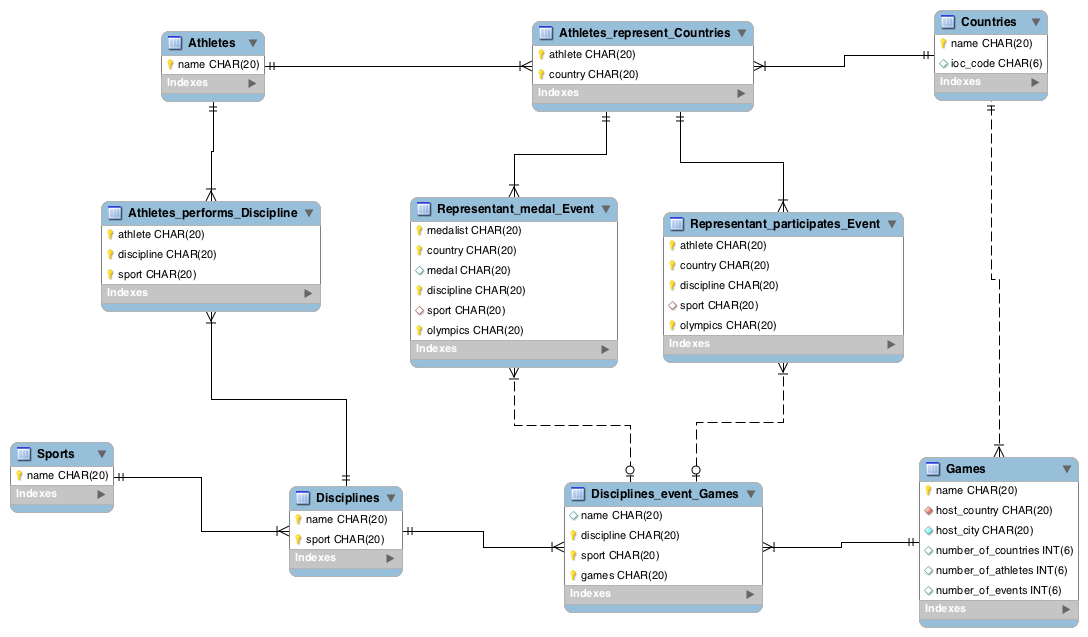
\includegraphics[width=0.9\textwidth]{ddl-scheme}}
	\caption{Generated EER Model from MySQL Workbench.\label{fig:ddl-scheme}}
\end{figure}
After implementing the DDL from Section \ref{sec:ddl}, we generated the scheme in Figure \ref{fig:ddl-scheme} using MySQL Workbench.

\section{SQL Data definition language statements}
\label{sec:ddl}

We decided to implement our project, using the Oracle MySQL database management system. Following is the listing of our entities and relations.

\begin{center}
	\lstinputlisting[caption={DDL Entities}]{sql/ddl-entities.sql}
\end{center}

\begin{center}
	\lstinputlisting[caption={DDL Relations}]{sql/ddl-relations.sql}
\end{center}


%------------------------------------------------------------------------------
% END OF DOCUMENT
%------------------------------------------------------------------------------